\chapter{Inflation, Vacuum Energy, and the de Sitter Mechanism}

Inflation is the announced subject of this lecture, but the lecturer does not begin there. He first rebuilds the simplest cosmological mechanism that will carry the whole story: if the energy density is a true vacuum energy, then it does not dilute; if it does not dilute, then the Hubble rate is constant; and if the Hubble rate is constant, then the scale factor grows exponentially. Only after that does he pivot to the present accelerated universe, the cosmic horizon, the quantum meaning of vacuum energy, and finally to the conjecture that the same de Sitter mechanism once operated in the remote past with a vastly larger effective vacuum energy. From there the lecture turns to a scalar field \(\phi\), its potential \(V(\phi)\), the slow drift along a high plateau, reheating at the cliff, and the survival of small quantum fluctuations that later become the seeds of galaxies.

\paragraph{Credit.} These companion notes follow Leonard Susskind's Lecture 7, with supporting frame extraction curated by LazyingArt LLC and Video2Book.

\section{Vacuum Energy, de Sitter Space, and Exponential Expansion}

The lecture opens by postponing inflation and going back to the Friedmann equation in flat space. Susskind speaks of \(A(t)\); here we use the standard \(a(t)\), with the same meaning:
\begin{equation}
\left(\frac{\dot a}{a}\right)^2=\frac{8\pi G}{3}\rho.
\end{equation}
The earlier cosmological cases are then recalled. For matter one has \(\rho\propto a^{-3}\); for radiation \(\rho\propto a^{-4}\); but for vacuum energy the density does not dilute at all:
\begin{equation}
\rho=\rho_0=\text{constant}.
\end{equation}
That is the special case he wants to isolate. If the right-hand side of the Friedmann equation is constant, we may write
\begin{equation}
H^2=\frac{8\pi G}{3}\rho_0,
\qquad
H=\sqrt{\frac{8\pi G}{3}\rho_0}.
\end{equation}
In this pure vacuum-energy cosmology the Hubble rate is truly constant:
\begin{equation}
\frac{\dot a}{a}=H.
\end{equation}
Now the differential equation is as simple as it can be:
\begin{equation}
\dot a = H a.
\end{equation}
Its solution is exponential,
\begin{equation}
a(t)=a_0 e^{Ht},
\end{equation}
so the distance between sufficiently separated unbound galaxies grows like \(e^{Ht}\). This exponentially expanding spacetime is de Sitter space.

The lecture also writes the metric in these expanding coordinates. Regularizing the spoken \(d\tau^2\) notation into the standard line element, we have
\begin{equation}
ds^2 = dt^2 - e^{2Ht}\left(dx^2+dy^2+dz^2\right).
\end{equation}
That is the basic machine. The later inflationary story will not introduce a different mechanism; it will re-use this one at a much larger scale.

One brief side issue appears here. The lecture assumes positive vacuum energy. In exactly flat space that is the case we need, because the left-hand side of the Friedmann equation is nonnegative. Negative vacuum energy can arise in more general cases once curvature terms are included, but that branch is not pursued in this lecture.

\begin{remark}
The lecture briefly recalls Einstein's original use of the cosmological constant as a balancing term against ordinary matter in an attempt to hold the universe static. It is worth remembering historically, but it is not part of the mathematical line we need here.
\end{remark}

\section{Present Acceleration and the Cosmic Horizon}

Having rebuilt pure de Sitter space, the lecture asks what use it has in cosmology. The first use is contemporary. The universe today is not exactly de Sitter, but it is moving in that direction. Earlier, the scale factor followed the matter-dominated law
\begin{equation}
a(t)\propto t^{2/3},
\end{equation}
whereas now the observed expansion bends upward toward an exponential.

\begin{figure}[h]
\centering
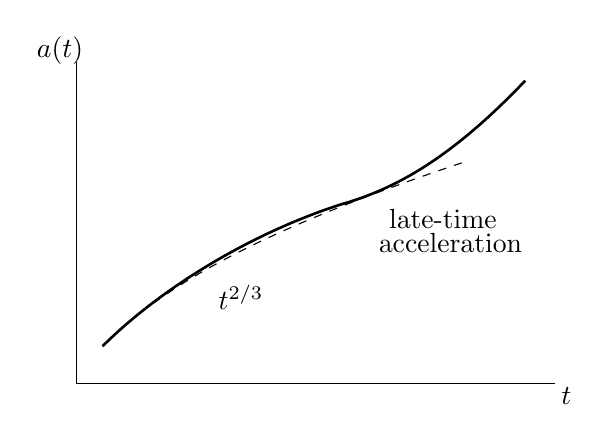
\begin{tikzpicture}[scale=0.95]
\draw (0,0) -- (6.4,0);
\draw (0,0) -- (0,4.3);
\node at (6.55,-0.16) {\(t\)};
\node at (-0.22,4.45) {\(a(t)\)};

\draw[dashed] (0.35,0.5) .. controls (1.1,1.25) and (2.3,2.0) .. (5.15,2.95);
\node at (2.2,1.15) {\(t^{2/3}\)};

\draw[line width=0.95pt] (0.35,0.5) .. controls (1.1,1.25) and (2.3,2.0) .. (3.55,2.4)
.. controls (4.25,2.6) and (5.0,3.0) .. (6.0,4.05);

\node at (4.9,2.2) {late-time};
\node at (5.0,1.88) {acceleration};
\end{tikzpicture}
\caption{The lecture's qualitative observational sketch: matter-dominated growth \(a(t)\propto t^{2/3}\) gives way at late times to accelerated expansion approaching an exponential.}
\end{figure}

Acceleration means exactly what it should mean:
\begin{equation}
\ddot a>0.
\end{equation}
The lecture insists that this is not a speculation. The late-time data do not yet give a perfect exponential, because the universe still contains other forms of energy, but the trend is clear: vacuum energy is beginning to dominate.

From there the lecture moves to the horizon. In proper-distance form, Hubble's law is
\begin{equation}
v=HD.
\end{equation}
The horizon is the distance at which the recession speed becomes the speed of light. Setting \(v=c\), we obtain
\begin{equation}
D=\frac{c}{H},
\end{equation}
or, equivalently,
\begin{equation}
HD=c.
\end{equation}
Only the first of these is fully secure from the board image; the second is the natural completion of the partially written line.

\begin{figure}[h]
\centering

\includegraphics[width=0.62\textwidth]{lecture_07_figure_02.png}
\caption{Hubble distance relation on the board. The right board cleanly shows \(D=c/H\); the upper line suggests the equivalent form \(HD=c\), while the left board preserves only a cropped residue of the preceding \(\rho_0\)-to-\(H\) discussion.}
\end{figure}

This figure matters for more than the equation itself. It preserves the lecture's board logic. On the left one is leaving the vacuum-energy derivation; on the right one has isolated the horizon formula. That is exactly the transition in the spoken argument.

\subsection{Question \& Answer}

Why is \(1/H\) numerically close to the age of the universe today, and why is that not a mathematical identity?

The lecture answers this by going back to a simple power law. If
\begin{equation}
a(t)=Ct^p,
\end{equation}
then
\begin{align}
\dot a &= Cp\, t^{p-1},\\
H=\frac{\dot a}{a} &= \frac{Cp\, t^{p-1}}{Ct^p}=\frac{p}{t}.
\end{align}
So only for the special case \(p=1\) do we get \(H=1/t\). For a matter-dominated universe,
\begin{equation}
p=\frac{2}{3},
\qquad
H=\frac{2}{3t}.
\end{equation}
Thus \(1/H\) is of the same order as the age, but not equal to it.

The point becomes sharper in exact de Sitter space. There \(H\) is constant while the age continues to increase, so \(1/H\) cannot possibly be the age of the universe. It is instead the e-folding time:
\begin{equation}
a(t+H^{-1})=e\,a(t).
\end{equation}
The lecturer says ``double'' a few times, but then corrects himself: the precise statement is multiplication by \(e\). The true doubling time would be
\begin{equation}
t_{\mathrm{double}}=\frac{\ln 2}{H}.
\end{equation}
So the near coincidence today between the horizon timescale and the age of the universe is contingent, not a mathematical identity. The lecture leaves it as a real question why these two scales happen to be comparable in the era in which we live.

\section{Vacuum Energy as Zero-Point Energy}

At this stage a student asks the obvious question: what is vacuum energy actually? That question is not brushed aside. It becomes the next teaching unit.

The lecture answers first in the language of ordinary quantum mechanics. Consider a harmonic oscillator. Suppressing inessential constants, its energy is written schematically as
\begin{equation}
E_{\mathrm{osc}}\sim p^2+x^2.
\end{equation}
Classically the ground state is the equilibrium point,
\begin{equation}
x=0,\qquad p=0,\qquad E=0.
\end{equation}
Quantum mechanically that state is forbidden by the uncertainty principle. One cannot simultaneously pin down position and momentum so sharply. Therefore the ground-state energy must be positive. For the harmonic oscillator one finds
\begin{equation}
E_0=\frac{1}{2}\hbar\omega.
\end{equation}

The lecture then lifts this picture from one oscillator to quantum fields. A field is full of modes, and each mode behaves like an oscillator. The electromagnetic field is used as the simplest example. Schematically, its energy density is
\begin{equation}
u_{\mathrm{EM}}\sim E^2+B^2.
\end{equation}
The treatment is pedagogical rather than canonical, but the point is clear. Even when there are no real photons in the field, the ground state is not a zero-energy state. There remain zero-point oscillations.

Every field has such modes, and every field contributes zero-point energy. That is one lecture-level explanation of vacuum energy. It is not yet an explanation of why the cosmological constant is so tiny. The lecture explicitly postpones that harder problem. For now it wants only the essential property: this energy is there, and as the universe expands it does not dilute.

\subsection{Question \& Answer}

How can ``empty'' space still carry energy?

Because the vacuum is not classical emptiness. It is the ground state of the quantum fields, and a quantum ground state need not have zero energy. The uncertainty principle forces irreducible fluctuations. So the vacuum can contain no ordinary particles and yet still carry zero-point energy.

The lecture also sharpens the distinction between vacuum energy and ordinary radiation. The three-degree microwave background is not vacuum energy. Radiation dilutes as the universe expands, and each photon redshifts as well. Vacuum energy is the residual field energy that remains even after all removable real quanta have been removed. That is why it does not dilute.

\section{Energy, Horizons, and What Stays Fixed in de Sitter Space}

Now the next objection arises. If the vacuum-energy density is constant while the universe expands, then does not the total vacuum energy increase? The lecture answers this cautiously and somewhat gesturally. It says, in effect, that in general relativity one is not dealing with ordinary mechanical energy alone; the expansion of space contributes a gravitational sector to the bookkeeping, and the concept of ``the energy'' is subtler than in elementary mechanics. It would be a mistake to convert this lecture comment into a polished Hamiltonian formula that was never actually derived on the board.

What the lecture does make precise enough is the horizon argument. In exact de Sitter space the horizon size is fixed:
\begin{equation}
D=\frac{c}{H}
=\frac{c}{\sqrt{8\pi G\rho_0/3}}.
\end{equation}
The volume inside that horizon is therefore fixed as well. If we estimate the vacuum energy accessible to a given observer, it scales like
\begin{equation}
E_{\mathrm{hor}}=\frac{4\pi}{3}D^3\rho_0.
\end{equation}
Since \(D\) is constant and \(\rho_0\) is constant, the amount of vacuum energy within the cosmic horizon does not change with time:
\begin{equation}
E_{\mathrm{hor}}=\text{constant}
\qquad
\text{(exact de Sitter space).}
\end{equation}

This is the lecture's practical answer. From the observer's standpoint, the portion of the universe that can ever be seen contains a fixed horizon volume and therefore a fixed amount of vacuum energy. The lecture also remarks that objects can pass through this horizon in much the same sense that they can pass through a black-hole horizon: once outside, they are no longer in causal contact with us.

\subsection{Question \& Answer}

If the vacuum-energy density is constant while space expands, where does the extra energy come from?

At the level of this lecture, the safest answer is: do not imagine a Newtonian box of ever-growing volume and then demand a simple conservation law for the energy inside that box. In exact de Sitter space the cosmic horizon is fixed, so the vacuum energy within the observable region is fixed. Beyond that, the lecture only wants to say that in general relativity the expansion sector participates in the bookkeeping, and that the idea of total energy is more delicate than in ordinary mechanics.

\section{Why Inflation Was Proposed}

Only after all of this does the lecture make its main turn. The same de Sitter mechanism, it says, appears to have operated in the remote past, but with a vastly shorter timescale:
\begin{equation}
H_{\mathrm{inf}}^{-1}\sim 10^{-32}\,\mathrm{s}.
\end{equation}
This is inflation. The universe in the remote past is conjectured to have undergone a period of exponential expansion before anything we can directly observe.

Why was such an idea introduced? The answer is not initially field-theoretic. It is geometric. The universe appears very flat and very homogeneous on large scales. More strikingly still, the surface of last scattering was already very smooth. So the smoothing cannot have happened only after the hot visible phase began. Something earlier must have stretched away the wrinkles.

The lecture's favorite analogy is the wrinkled balloon. Start with a completely deflated balloon and it is full of folds and texture. Inflate it enough and any local patch becomes nearly smooth. The raisin or prune analogy serves the same purpose. A wrinkled object, if stretched enormously, looks smooth on any visible patch. That is the intuition behind inflation.

The horizon problem then enters naturally. We see distant regions of the last-scattering surface that could not have exchanged signals with one another in the available time. So why do they have nearly the same density and temperature? Inflation answers by proposing a prehistory to what we ordinarily call the Big Bang: an earlier phase of exponential expansion stretches one small region into something vastly larger than the present observable universe.

The lecture is quite candid about the mixed blessing here. The good thing about inflation is that it erases the initial conditions. One need not know the detailed prehistory in order to explain why the visible universe is so smooth. The bad thing is the same: inflation erases much of the information about how things started.

This is also where the lecture reconnects with spatial curvature. Observationally the universe appears spatially flat, with the curvature parameter \(k\) consistent with zero to very good accuracy. Inflation explains why that should be so. If the universe expanded enough before the visible hot era, then the curvature radius became so large that the region we can see now looks Euclidean.

\section{Scalar Field \(\phi\) and the Potential \(V(\phi)\)}

So far inflation has been motivated geometrically. The next question is what could have supplied the much larger effective vacuum energy in the remote past. That is the point at which the scalar field enters.

A scalar field \(\phi\) is a field with no directionality. At each point in space and time it simply takes a value:
\begin{equation}
\phi=\phi(x,y,z,t).
\end{equation}
The lecture emphasizes that this is a hypothetical field. It is not identified with any known particle or any familiar observed field. It is introduced because the mathematics allows it and because the inflationary story seems to ask for something like it.

What matters is its potential-energy density \(V(\phi)\). This is energy associated with the field value itself, not with the time derivative of the field. Different values of \(\phi\) may carry different potential energies.

\begin{figure}[h]
\centering

\includegraphics[width=0.68\textwidth]{lecture_07_figure_03.png}
\caption{The first scalar-potential sketch used in the lecture. The board notation \(V(\phi)\) is visible, and the curve makes the essential point that different values of \(\phi\) correspond to different potential energies.}
\end{figure}

\begin{figure}[h]
\centering
\begin{tikzpicture}[scale=0.95]
\draw (0,0) -- (6.3,0);
\draw (0,0) -- (0,4.25);
\node at (6.45,-0.15) {\(\phi\)};
\node at (-0.16,4.4) {\(V\)};

\draw[line width=0.95pt]
(0.35,3.55) .. controls (1.1,1.9) and (1.55,1.35) .. (2.15,1.52)
.. controls (2.8,1.75) and (3.25,3.45) .. (4.1,3.28)
.. controls (4.75,3.16) and (5.15,1.65) .. (5.85,1.0);
\end{tikzpicture}
\caption{A clean redraw of the lecture's generic \(V(\phi)\) sketch. At this stage the point is simply that the potential energy changes with the field value.}
\end{figure}

Now comes the decisive identification. If \(\phi\) is approximately constant over the region we are studying, then \(V(\phi)\) behaves just like vacuum energy:
\begin{equation}
\rho_{\mathrm{eff}}=V(\phi).
\end{equation}
Therefore the earlier de Sitter formula can be reused with the simple replacement
\begin{equation}
\rho_0 \longrightarrow V(\phi).
\end{equation}
The corresponding Hubble rate is then
\begin{equation}
H(\phi)=\sqrt{\frac{8\pi G}{3}V(\phi)}.
\end{equation}

This is the mathematical bridge between the first half of the lecture and the second. Inflation is not some additional cosmological law glued onto the Friedmann equation. It is the same Friedmann equation read with a different source.

The lecture then asks what happens if \(\phi\) varies from place to place. In that case different regions expand with different local time constants. But exponential stretching tends to make any visible patch look more and more homogeneous. That is why inflation can start with a field that is only approximately uniform and still leave us living in a region where it appears nearly constant.

\subsection{Question \& Answer}

What are the axes of the \(V(\phi)\) graph, and in what sense can \(\phi\) behave like a time parameter without being time itself?

The horizontal axis is the field value \(\phi\), and the vertical axis is the potential-energy density \(V\). So this is not a graph of energy against time. It is a graph of energy against field value.

But if \(\phi\) rolls monotonically down the potential, then the successive values of \(\phi\) label successive moments along the cosmological history. In that restricted sense \(\phi\) can act like a time parameter: later times correspond to later values along the curve. Still, \(\phi\) is not time itself. It is a field value whose evolution happens to be monotonic during the relevant epoch.

\section{Reheating, E-foldings, and Primordial Fluctuations}

The lecture now sharpens into the picture it regards as observationally demanded. The potential is high on the left, almost flat over a broad plateau, then it comes to a cliff, falls sharply, and settles into a lower minimum which is not exactly at zero.

\begin{figure}[h]
\centering

\includegraphics[width=0.68\textwidth]{lecture_07_figure_04.png}
\caption{The inflationary potential as drawn late in the lecture: a high plateau, a sharp drop, and a lower minimum.}
\end{figure}

\begin{figure}[h]
\centering
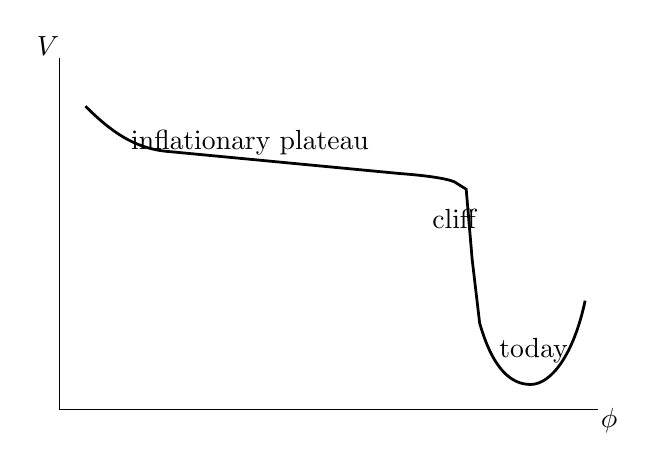
\begin{tikzpicture}[scale=0.95]
\draw (0,0) -- (7.2,0);
\draw (0,0) -- (0,4.7);
\node at (7.35,-0.15) {\(\phi\)};
\node at (-0.15,4.85) {\(V\)};

\draw[line width=1pt]
(0.35,4.05) .. controls (0.7,3.7) and (1.0,3.5) .. (1.4,3.45)
-- (4.55,3.15)
.. controls (4.95,3.12) and (5.18,3.08) .. (5.28,3.04)
-- (5.44,2.94)
-- (5.52,2.0)
-- (5.62,1.15)
.. controls (5.8,0.52) and (6.05,0.33) .. (6.3,0.33)
.. controls (6.58,0.33) and (6.88,0.74) .. (7.03,1.45);

\node at (2.55,3.56) {inflationary plateau};
\node at (5.28,2.55) {cliff};
\node at (6.34,0.78) {today};
\end{tikzpicture}
\caption{A schematic redraw of the lecture's high-plateau, cliff, and minimum structure. The large-scale shape, not the exact marker trace, is what matters.}
\end{figure}

The lecture is careful not to pretend that this is derived from first principles. It calls the picture contrived, even ridiculous-looking, but says that observational cosmology seems to demand something like it.

Now the inflationary stage becomes very vivid. High on the plateau the field moves slowly, because the slope is small and the cosmological friction is large. The lecture insists that the right analogy is viscosity rather than ordinary stick-slip friction. A rock falling slowly through honey is closer to the picture than a block on a rough table. The faster the universe expands, the larger this effective cosmological viscosity becomes. So the field drifts only very slowly:
\begin{equation}
\text{small slope} + \text{large cosmological viscosity}
\quad \Longrightarrow \quad
\phi \text{ drifts slowly}.
\end{equation}
While that happens, \(V(\phi)\) changes only a little, so the expansion remains approximately exponential. That is the inflationary phase.

The lecture then turns this into a quantitative timescale. If the scale factor changes from \(a_i\) to \(a_f\), the number of e-foldings is
\begin{equation}
N=\ln\frac{a_f}{a_i}.
\end{equation}
One e-fold means multiplication by \(e\). The lecture gives a lower bound of roughly fifty e-foldings, while noting that sixty is the standard figure often quoted:
\begin{equation}
N\gtrsim 50,
\qquad
N\sim 60 \ \text{as the usual benchmark.}
\end{equation}
The e-folding time during inflation is of order
\begin{equation}
H_{\mathrm{inf}}^{-1}\sim 10^{-32}\,\mathrm{s}.
\end{equation}
The lecture also gives, cautiously, a rough ballpark for the plateau height, of order \(10^{-14}\) in Planck units, though only as an estimate at the level of bounds.

At the bottom of the potential the geometry tells us the remaining vacuum energy today. Since
\begin{equation}
H^2=\frac{8\pi G}{3}V,
\end{equation}
the present minimum satisfies
\begin{equation}
V_{\mathrm{today}}=\frac{3H_0^2}{8\pi G},
\end{equation}
while on the inflationary plateau one had
\begin{equation}
V_{\mathrm{inf}}=\frac{3H_{\mathrm{inf}}^2}{8\pi G}\gg V_{\mathrm{today}}.
\end{equation}
This is the lecture's way of reading the board sketch quantitatively: the top was much higher, the bottom is small but not zero.

Now the field reaches the cliff. Its potential energy turns into kinetic energy of motion, and then into heat, radiation, and particles. The lecture calls this reheating, while half-apologizing for the name. There is nothing particularly ``re'' about it unless one speculates about an even earlier prehistory. The essential point is that the universe is not hot on the plateau. Any pre-existing heat would have been diluted away by inflation. It becomes hot only after the fall.

This is also where the lecture deliberately plays with the phrase ``Big Bang.'' One may, if one likes, speak of reheating as the Big Bang in a prehistory sense. But the visible Big Bang of ordinary cosmological language is much later. The surface of last scattering comes only after the universe has cooled enough to become transparent. In the lecture's potential sketch, everything we actually observe lies down near the bottom.

\subsection{Question \& Answer}

Why must the plateau not be perfectly flat, and how do the remaining fluctuations become structure?

If the plateau were exactly flat, the field would have no classical force pushing it along. The lecture therefore insists that the plateau is not perfectly flat. It must have some tilt. At the same time it cannot be too steep, or inflation would end too quickly. So one already sees a balance: enough tilt to move, little enough tilt to linger.

But there is a second balance. If the field moves too slowly for too long, then small quantum differences from one place to another become large differences in the times at which different regions reach the cliff. That would make the reheated universe too inhomogeneous. So the observed smallness of the primordial fluctuations constrains the flatness and height of the potential. The lecture is explicit about this: the observed \(\delta\rho/\rho\sim 10^{-5}\) does not drop out of the qualitative picture automatically; it constrains the parameters of the picture.

The late part of the lecture then gives the central diagram. One plots ordinary space vertically and the field value \(\phi\) horizontally. Surfaces of constant field are like contour lines on a map. If the field were perfectly homogeneous, those contours would be straight, and every region would fall over the edge together. Quantum mechanics spoils that exact homogeneity.

\begin{figure}[h]
\centering
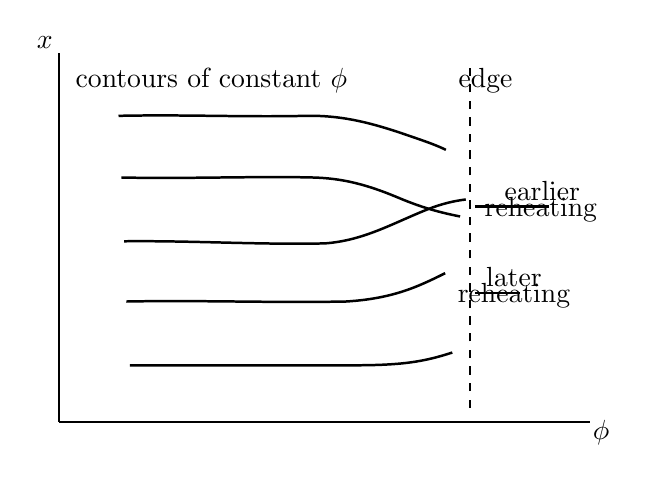
\begin{tikzpicture}[scale=0.9]
\draw (0,0) -- (7.5,0);
\draw (0,0) -- (0,5.2);
\node at (7.65,-0.15) {\(\phi\)};
\node at (-0.2,5.35) {\(x\)};

\draw[dashed] (5.8,0.2) -- (5.8,5.0);
\node at (6.02,4.82) {edge};

\draw[line width=0.9pt] (1.0,0.8) .. controls (2.0,0.8) and (3.2,0.8) .. (4.15,0.8)
.. controls (4.85,0.8) and (5.15,0.85) .. (5.55,0.98);

\draw[line width=0.9pt] (0.95,1.7) .. controls (2.0,1.72) and (3.0,1.68) .. (4.05,1.7)
.. controls (4.7,1.74) and (5.05,1.9) .. (5.45,2.1);

\draw[line width=0.9pt] (0.92,2.55) .. controls (1.9,2.56) and (2.8,2.5) .. (3.75,2.52)
.. controls (4.3,2.56) and (4.7,2.8) .. (5.2,3.0)
.. controls (5.4,3.08) and (5.58,3.12) .. (5.74,3.14);

\draw[line width=0.9pt] (0.88,3.45) .. controls (1.8,3.43) and (2.8,3.47) .. (3.58,3.45)
.. controls (4.0,3.44) and (4.35,3.35) .. (4.8,3.16)
.. controls (5.18,3.0) and (5.46,2.94) .. (5.66,2.9);

\draw[line width=0.9pt] (0.84,4.32) .. controls (1.78,4.34) and (2.6,4.3) .. (3.48,4.32)
.. controls (3.95,4.33) and (4.34,4.24) .. (4.82,4.08)
.. controls (5.08,3.99) and (5.3,3.92) .. (5.46,3.84);

\draw[line width=1pt] (5.87,3.04) -- (6.92,3.04);
\draw[line width=1pt] (5.87,1.82) -- (6.5,1.82);

\node at (2.15,4.82) {contours of constant \(\phi\)};
\node at (6.82,3.26) {earlier};
\node at (6.8,3.0) {reheating};
\node at (6.42,2.05) {later};
\node at (6.42,1.79) {reheating};
\end{tikzpicture}
\caption{A transcript-driven contour sketch. Small quantum bumps in the field make different regions reach the cliff at different times, and those time delays become density inhomogeneities after reheating.}
\end{figure}

The lecture likes to describe this in several equivalent ways. One may imagine a little bump in an otherwise homogeneous field. One may imagine soldiers walking in lockstep toward a cliff, some a little ahead, some a little behind. Either way, the result is the same: some regions fall over earlier, others later.

Now the key point. The region that falls earlier reheats earlier and then has more time to expand and cool. The region that falls later is reheated later and remains hotter and denser. That is how a tiny fluctuation in \(\phi\) becomes a fluctuation in energy density. The lecture summarizes the observed amplitude as
\begin{equation}
\frac{\delta\rho}{\rho}\sim 10^{-5}.
\end{equation}
These are primordial density fluctuations, not dark energy. They are small, but without them there would be no galaxies.

After reheating, gravity amplifies them further. Over-dense regions attract more material; under-dense regions are depleted. So the tiny initial contrasts are magnified into the structure we see. The lecture stresses that this is not just a qualitative story. One can compute the fluctuation spectrum from quantum fields in an expanding background and compare it with the reconstructed primordial spectrum inferred from galaxies and the microwave background. The lecture's verdict is strong: it fits very well.

And then the final pivot. These fluctuations do not just seed galaxies. They are processed into acoustic waves in the primordial plasma, and those acoustic waves provide a standard ruler on the sky. That ruler will be the subject of the next lecture, where geometry is measured from the angle subtended by structures of known physical size on the last-scattering surface.

\section{Summary}

The lecture begins by refusing to begin with inflation. Instead it rebuilds the de Sitter mechanism in its simplest form: constant vacuum-energy density implies constant \(H\), and constant \(H\) implies
\[
a(t)=a_0 e^{Ht}.
\]
That mechanism is then used twice. First, to understand the present accelerated universe and the horizon scale \(D=c/H\). Second, to motivate the idea that a much earlier de Sitter-like phase may have occurred in the remote past.

The student questions are not side remarks; they are part of the structure. They force the lecture to explain vacuum energy as zero-point energy and to think carefully about what stays fixed inside a de Sitter horizon. Only then does the main inflationary picture arrive. A hypothetical scalar field \(\phi\) with potential \(V(\phi)\) sits high on a nearly flat plateau, drifts slowly under a small slope and cosmological viscosity, falls off a cliff, reheats the universe, and finally settles near a low but nonzero minimum whose leftover energy is today's dark-energy-like vacuum energy.

The lecture's deepest payoff comes at the end. Inflation smooths the universe, but quantum mechanics prevents complete uniformity. Different regions reheat at slightly different times, producing primordial density contrasts of order \(10^{-5}\). Gravity then amplifies those contrasts into galaxies, while the microwave background preserves their early imprint. So the same mechanism that wipes out the initial wrinkles also leaves behind the small residue from which structure grows.